\section{Countermeasures and Their Usage}
\label{sec:countermeaseres}

To mitigate the attacks previously shown we have to apply some preventive countermeasures. It can be useful to use the handler that is stopping some pods when a suspicious behavior is detected, but our primary goal is to be sure the attacks cannot occur in the first place. We analyzed two tools that are provided with Kubernetes, so there is no need to install anything. They are \acrlong{psa} and Seccomp. The first one is used to control pods when they are created, the other one is controlling the system calls made by a pod. It is worth noting that we know that there are also other tools such as Kyverno (YAML based) and Gatekeeper (Rego based) that control pods on admission in a similar way to \ac{psa} but with more granular policies and without the need of a dedicated namespace. They work in the same way as Falco and Tracee, deployed as deployments in the cluster with permission on that. Let's now focus on the tools that we actually used.


\subsection{Pod Security Admission}
\Acrlong{psa} is an admission controller that is provided with Kubernetes. It has been introduced in Kubernetes v1.22 and it enforces predefined Pod Security Standards at namespace level. The three namespaces (Privileged, Baseline and Restricted) are applying an increasing level of security and they define which configurations are allowed for a pod to enter. The requirements are the following:
\begin{itemize}
    \item Privileged: this namespace has no restrictions and allows all type of privilege and behavior;
    \item Baseline: to enter here we want no privilege containers, no host namespaces, no unsafe volume types, no sensitive capabilities and no Seccomp disabled;
    \item Restricted: for this last namespace requires all the baseline adding no root users, a read-only file system, drop all capabilities, mandatory to set a Seccomp profile and not allow privilege escalation.
\end{itemize}
\Ac{psa} acts when pod resources are created or updated, rejecting those that violate policies assigned for that namespace.

Since \ac{psa} is native to Kubernetes, it is simpler to manage than external tools like Kyverno or Gatekeeper when we don't want to introduce third-party components in our cluster. Policies are applied using a label in the namespace that specifies the enforcement level:

e.g. \texttt{pod-security.kubernetes.io/enforce: restricted}

\noindent Other modes like audit and warn (replacing enforce) are non-blocking and used only for monitoring.

\Ac{psa} is limited to the pod-level and provides a lightweight mechanism to avoid misconfigured workloads in the cluster. This can be considered a first line defense because it ensures that deployed workloads meet a minimum security threshold without additional tools.


\subsubsection{Application of PSA}
\Ac{psa} policies have been applied in our project creating a new namespace named \texttt{secured}. We added the specific label that is needed to make that namespace a Restricted one.

When the namespace is created we have to edit the deployment for the application. We need to use a non-root user in the image, use the default Seccomp policy, remove capabilities and disallow privilege escalation. Finally the pod is deployed in the new \texttt{secured} namespace. If any of these options is not set, it will result in the pod not being deployed and causing an error in startup. All these actions are already set in \texttt{scenario/manifests/zipapp-deployment-psa.yaml}. The scenario secured with \ac{psa} can be deployed with:

\texttt{bash scenario/zipapp-psa-start.sh}

\noindent This will protect from the attack that we called "Dropped Executable"; others are still working and require other countermeasures that we will explain in a while.


\subsubsection{Effects on Dropped Executable Attack}
After deploying this new updated application we can notice that everything is still working as before if we try to perform any ordinary action on the website. When the "Dropped Executable" attack is performed the website shows "Internal Server Error" like shown in \autoref{fig:error} instead of a timeout message (\autoref{fig:timeout}), indicating that certain types of error happened during execution of the \texttt{zip} command. This is because the limited permission given in this new container are blocking commands like \texttt{apt update} or installation of new tools to download binaries from the Internet. If no tools to download like \texttt{wget} or \texttt{curl} are included in the base image this is enough to block this kind of attack. Finally if we try to log Falco using:

\texttt{bash falco-conf/falco-logs.sh}

\noindent or Trace with:

\texttt{bash tracee-conf/tracee-logs.sh}

\noindent or their respective event handler we will notice that there is no alert about the event that was triggered before. This means that the attack is no more performed thanks to the \ac{psa} countermeasure.

\begin{figure}[H]
    \centering
    \fbox{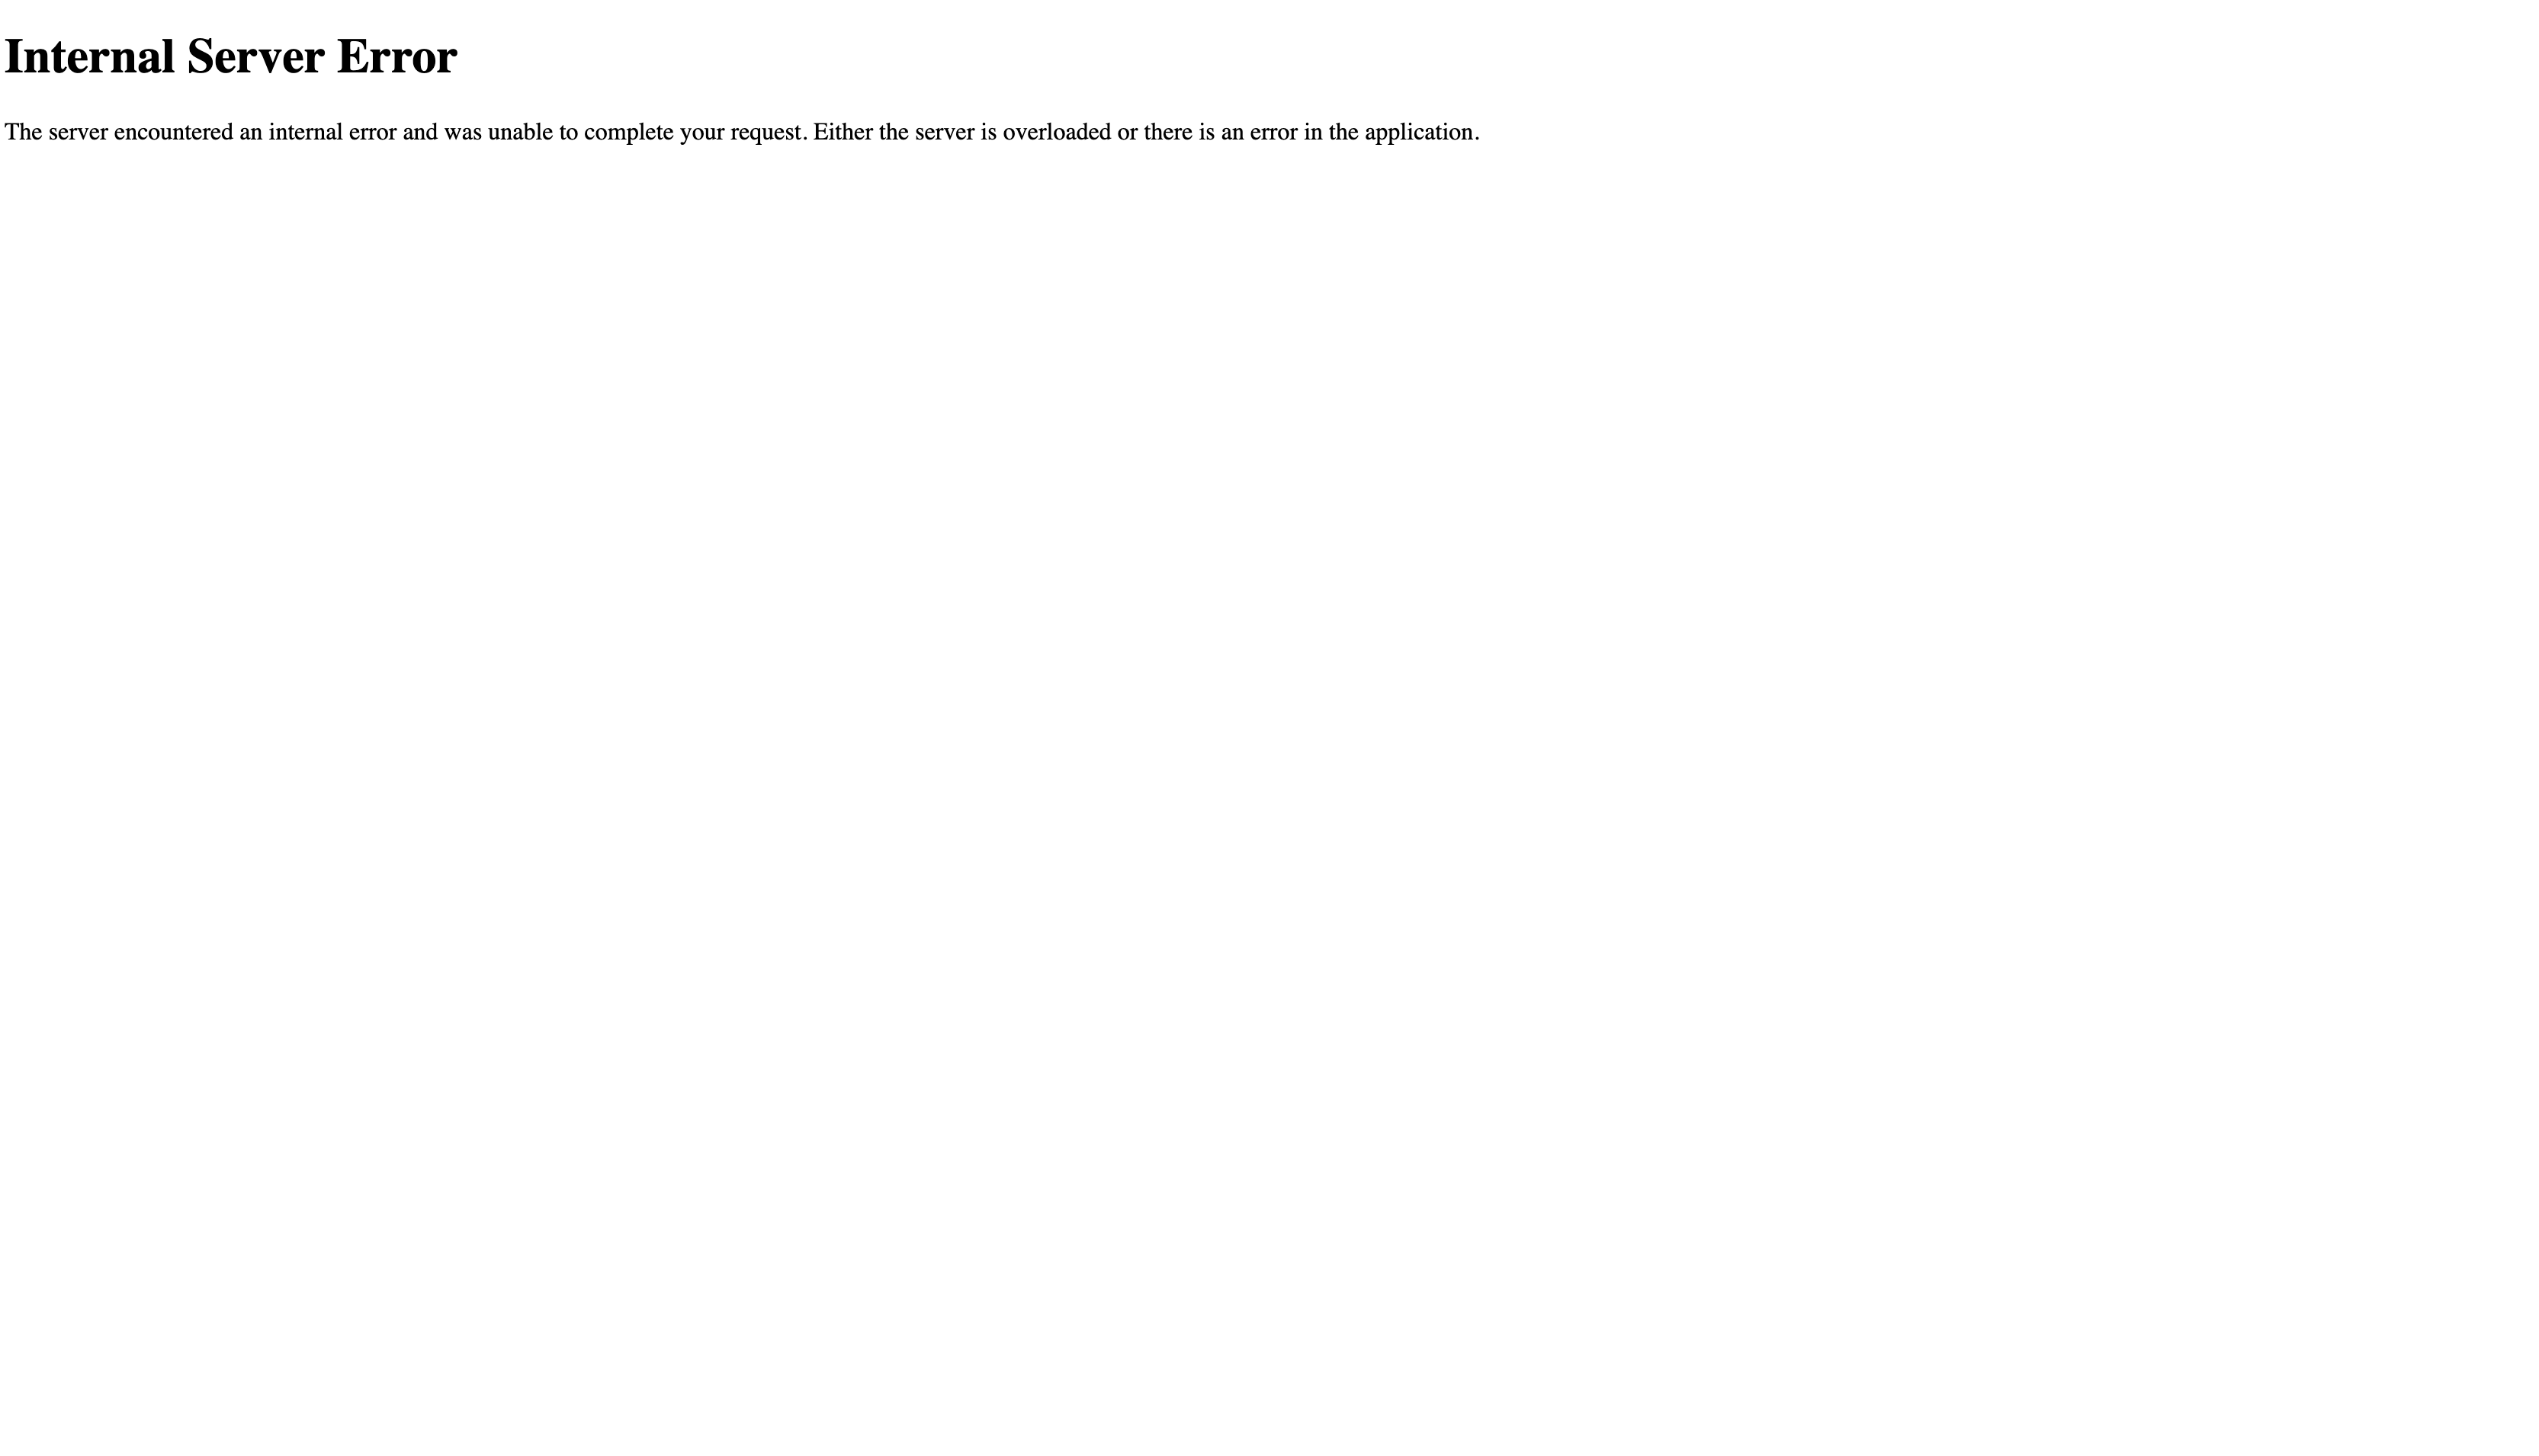
\includegraphics[width=0.70\linewidth]{images/error.png}}
    \caption{Screen of the WebApp in Error When the Attack is Blocked}
    \label{fig:error}
\end{figure}


\subsection{Seccomp}
Seccomp (short for Secure Computing Mode) is a feature that can be found in general in the Linux kernel. It is not specific of Kubernetes environment but it is very useful if applied to it. It is a lightweight mechanism used to reduce kernel attack surface within a container. A Seccomp profile is a JSON or YAML file where we can define which system calls are allowed or not. When a system call is not allowed we can return an error or kill the process that generated it. This mechanism is useful because some attacks in particular leverage on specific system calls which are rarely used in normal applications.

Seccomp in Kubernetes can be applied using the "securityContext.seccompProfile" property in pod specification through YAML file. With "RunTimeDefualt" we are using the default profile provided with the container. Otherwise we can create a custom one, like we did to contain simulated attacks about Reverse Shell and Ptrace Execution. In general, usage of Seccomp with very restricted policies is reserved to expert users, because it can result in problems if the wrong system call is blocked. We used it in a very basic way to demonstrate its working mechanism and to block attacks based on a single system call. Blocking attacks like the one about the "Dropped Executable" can become very risky and complex because deep knowledge of application behavior is required.

Seccomp can become also part of \ac{psa} because, as cited before, we can have some namespaces where a policy is required. This Linux kernel tool is very useful to implement the least privilege mechanism at the syscall level, to contain also potential compromised containers.


\subsubsection{Application of Seccomp}
We applied Seccomp to the reference scenario adding a custom profile. We prepared a pair of profiles that can be applied in every namespace (even the default one) and without the need of \ac{psa}.

First of all we need to copy the Seccomp profile needed inside Minikube to be loaded in the K8s application container. It is added to the YAML configuration of the deployment. Now we can start the deployment and the service. In particular we have a policy that allows everything except the \texttt{connect} syscall that is used to establish a network connection to block "Reverse Shell" attack and another one that blocks \texttt{ptrace} system call for the "Ptrace Execution" attack. They can be found in the folder \texttt{scenario/sec-profiles/}. When these are executed the kernel returns an error. The commands for deployment are:

\texttt{bash scenario/zipapp-seccomp-ptrace-start.sh}

\noindent for the one about Ptrace and:

\texttt{bash scenario/zipapp-seccomp-revshell-start.sh}

\noindent for the one about Reverse Shell. Note that if any malicious process performs an attacks without these syscalls it will succeed without any problem, but it will noticed by Falco or Tracee.


\subsubsection{Effects on Reverse Shell and Ptrace Attacks}
When these countermeasures are applied, like before everything is working properly and the application is behaving as expected. When we run both the attacks, we get as a response the "Internal Server Error" from \autoref{fig:error}. The error given by Seccomp is propagated back to the \texttt{zip} command that is executing the malicious executable. This results in incomplete action and no files will be zipped for download. Checking logs of Falco:

\texttt{bash falco-conf/falco-logs.sh}

\noindent or Trace with:

\texttt{bash tracee-conf/tracee-logs.sh}

\noindent or their respective event handler we will notice that there is no alert about the event that was triggered before. This means that the attack is no more performed thanks to the Seccomp countermeasure.

